\section{Grafi di test}
Dopo l'implementazione degli algoritmi descritta nel capitolo 4, è stato fatto un test con alcuni grafi arbitrariamente costruiti. Come prima cosa, vengono generati manualmente 4 grafi che rappresentano alcuni degli schemi di catene che potrebbero verificarsi all'interno del tx-graph.

Il primo schema rappresenta il classico cammino dritto, e si può notare in figura \ref{fig:straightgraph}. All'esecuzione dell'algoritmo, viene stampato il path = [0,1,2,3,...,9].
\begin{figure}[htbp]
	\centering
	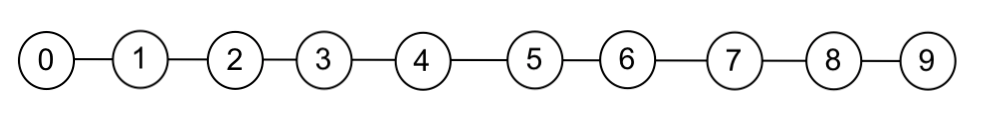
\includegraphics[width = \linewidth]{figure/straightgraph}
	\caption{\textit{Un cammino}\label{fig:straightgraph}}
\end{figure}
Nella figura \ref{fig:ygraph} si può notare un grafo a forma di Y, ovvero due cammini che convergono sullo stesso nodo. Potrebbe essere un classico esempio di una situazione di "merge".
\begin{figure}[htbp]
	\centering
	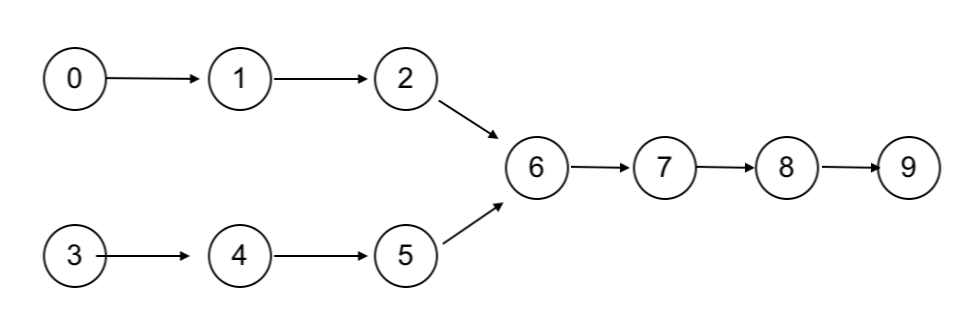
\includegraphics[width = \linewidth]{figure/ygraph}
	\caption{\textit{Un Y grafo}\label{fig:ygraph}}
\end{figure}
Nella fase di test su questo tipo di grafo, tra il nodo 2 e il nodo 5, il nodo 2 ha varianza minore, e il path restituito dall'algoritmo corrisponde proprio a [0,1,2,6,7,8,9].

Nella figura \ref{fig:xgraph} si ha un nuovo schema di grafo a forma di X. Se si esegue l'algoritmo anche su questo, a parità di varianza dei cammini, si otterrà come risultato il path [0,1,2,3,4,5], che è il più lungo.
\begin{figure}[htbp]
	\centering
	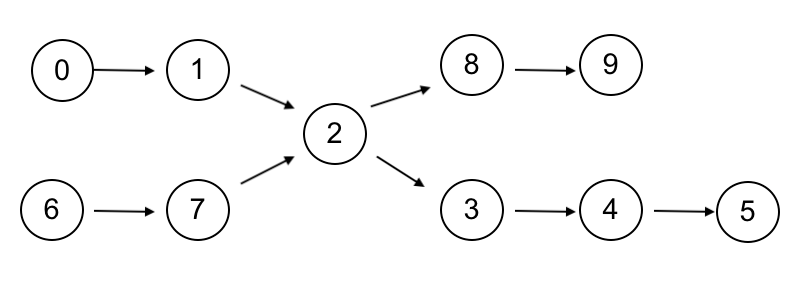
\includegraphics[width = 0.8\linewidth]{figure/xgraph}
	\caption{\textit{Un X grafo}\label{fig:xgraph}}
\end{figure}

Per quanto l'algoritmo del calcolo del cammino più lungo a varianza minima si corretto, a parità di cammini di eguale lunghezza ed egual varianza, stampa solamente il primo di essi, tralasciando gli altri cammini equivalenti.

\section{MatPlotLib per i grafici}
Dopo l'esecuzione dell'algoritmo, quindi, ogni nodo viene etichettato con attributi di frequenza(sia istantanea che media) e varianza. La frequenza istantanea non è molto rilevante per quanto riguarda lo studio sul tx-graph. 

Perciò si è deciso di graficare la distribuzione di tali valori su dei grafici con istogrammi, fatti con una libreria di python chiamata \textbf{MathPlotLib}. I grafici ottenuti rappresentano, sull'asse x la distribuzione dei singoli valori di frequenza(o varianza) dei nodi, e sull'asse y quanti sono quei nodi che hanno tale valore di frequenza(o varianza).

\section{Statistiche \& Grafici}
Inizialmente si è voluto graficare il primo dataset D1(417113, 417256), perchè è quello che più semplicemente si presta a generare un grafico attendibile. Nella figura \ref{fig:histg1} si può notare l'istogramma del primo dataset.
\begin{figure}[htbp]
	\centering
	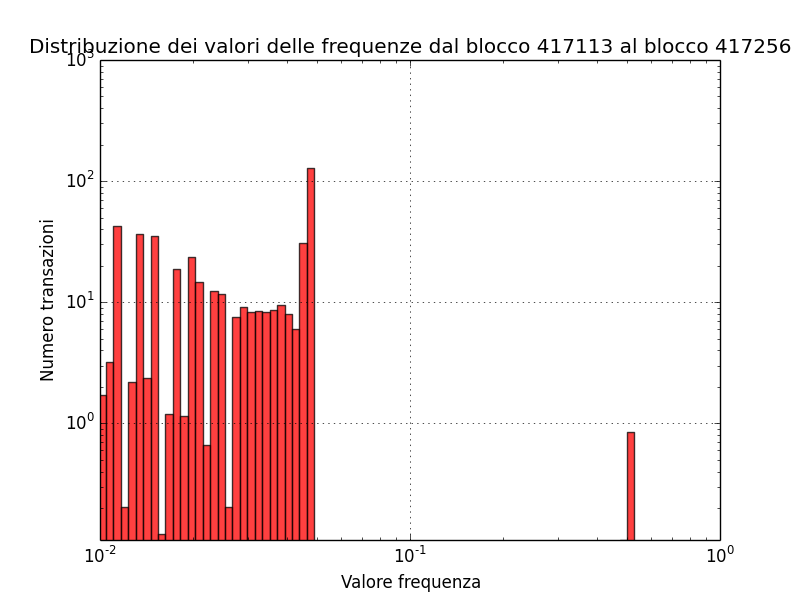
\includegraphics[width = 0.8\linewidth]{figure/histg1}
	\caption{\textit{G1(417113, 417256)}\label{fig:histg1}}
\end{figure}
\newpage
\subsection{Al variare del Dataset}
Prendendo successivamente in considerazione il dataset D2(413000, 414000), e di conseguenza il grafo generato da tale dataset, si è preferito creare dei grafici al variare della dimensione del dataset, per vedere quali erano i valori che si sarebbero aggiunti alla distribuzione.

Nelle figure seguenti, si potranno vedere i grafici creati dalla distribuzione dei valori di frequenza, al variare della dimensione dell'input, ovvero del numero di blocchi processati. In figura \ref{fig:hist20b} il grafico viene fatto su 20 blocchi, e si può notare come abbia un andamento decrescente e infine un picco.

\begin{figure}[htbp]
	\centering
		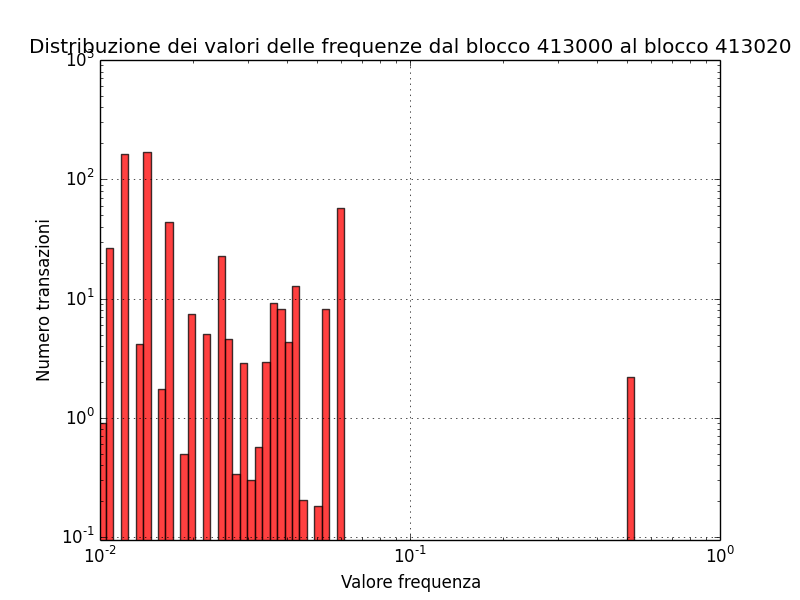
\includegraphics[width=0.7\textwidth]{figure/hist20b}
		\caption{\textit{20 blocchi}\label{fig:hist20b}}
\end{figure}
	
\begin{figure}[htbp]
	\centering
		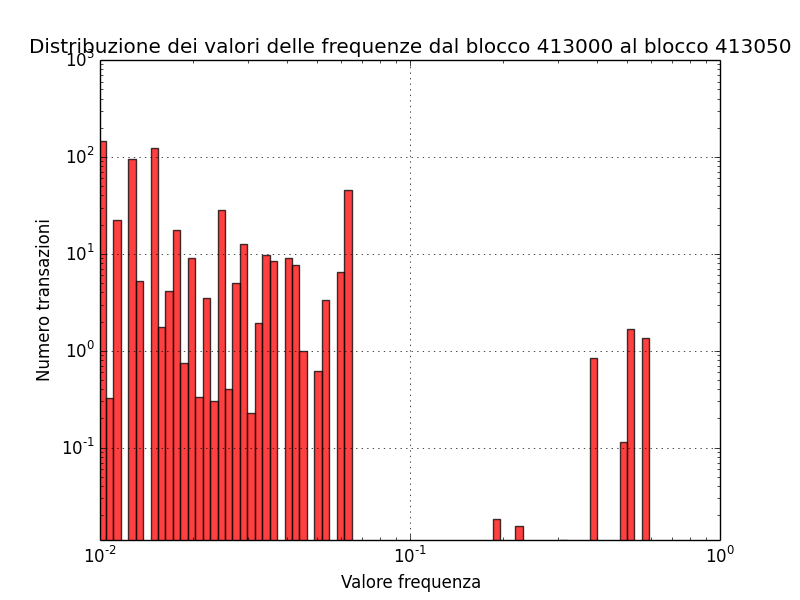
\includegraphics[width=0.7\textwidth]{figure/hist50b}
		\caption{\textit{50 blocchi}\label{fig:hist50b}}
\end{figure}

\begin{figure}[htbp]
	\centering
		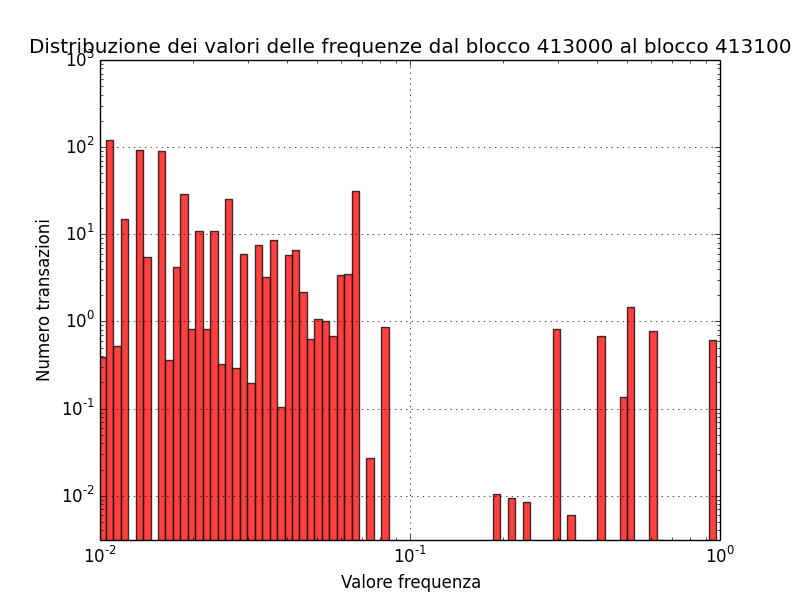
\includegraphics[width=0.7\textwidth]{figure/hist100b}
		\caption{\textit{100 blocchi}\label{fig:hist100b}}
\end{figure}
	
\begin{figure}[htbp]
	\centering
	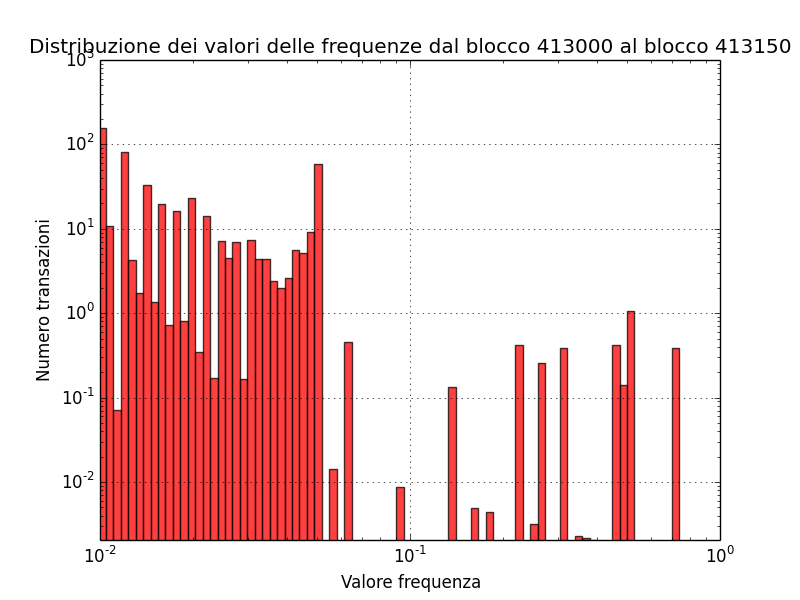
\includegraphics[width=0.7\textwidth]{figure/hist150b}
	\caption{\textit{150 blocchi}\label{fig:hist150b}}
\end{figure}

\begin{figure}[htbp]
	\centering
	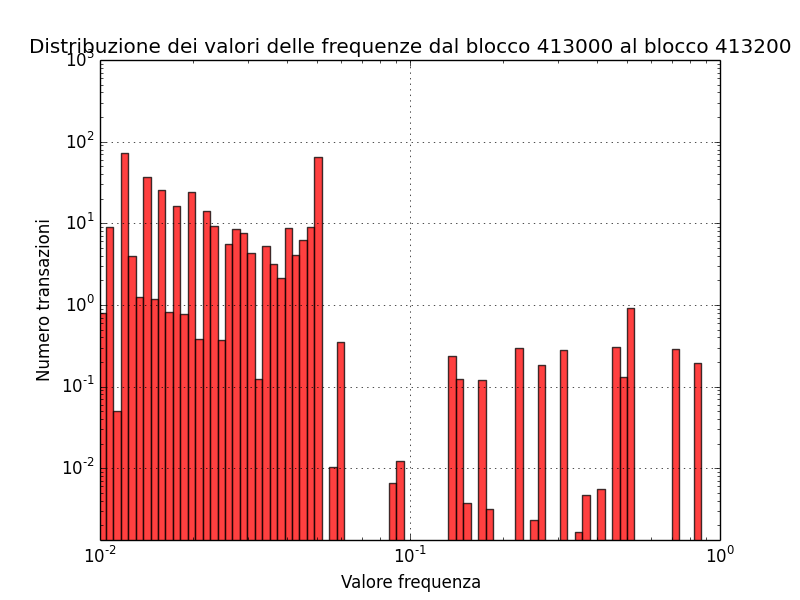
\includegraphics[width=0.7\textwidth]{figure/hist200b}
	\caption{\textit{200 blocchi}\label{fig:hist200b}}
\end{figure}

\begin{figure}[htbp]
	\centering
	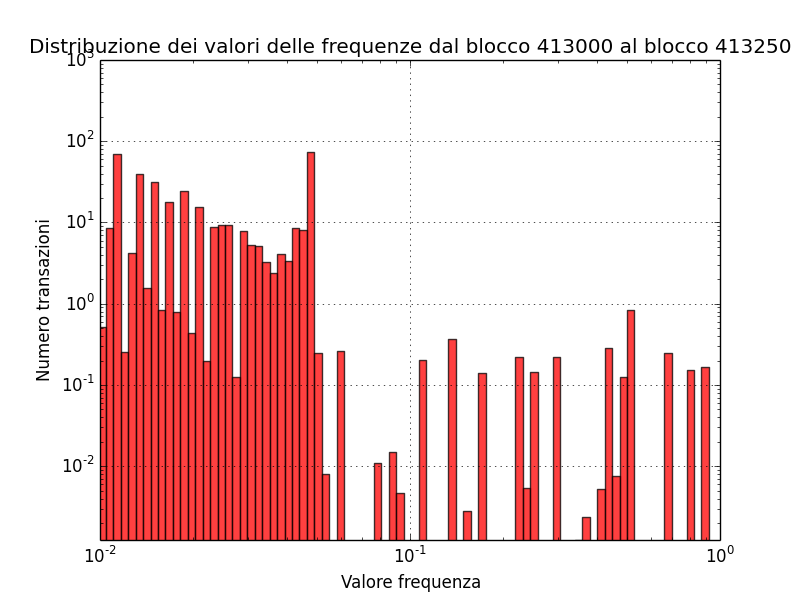
\includegraphics[width=0.7\textwidth]{figure/hist250b}
	\caption{\textit{250 blocchi}\label{fig:hist250b}}
\end{figure}
\newpage
Con l'aumentare del numero di blocchi, la parte destra del grafico va a riempirsi di ulteriori valori. Infatti, è sempre presente un andamento decrescente sulla sinistra, e dopo la decrescita, si ha una stabilità di valori sulla destra. Perciò, con il variare della grandezza del dataset, il numero di valori aumenta, ma l'andamento rimane sempre lo stesso.

Nell'ultimo grafico, in \textit{figura \ref{fig:hist1000b}}, si può notare un tratto decrescente e poi una stabilità di valori, che mediamente mantengono lo stesso andamento. Si può quindi osservare che valori di frequenza più piccoli di $10_{-1}$ seguono una retta decrescente, con un picco finale e la decrescita si interrompe di colpo dando spazio agli altri valori.

Si sono messi a confronto i grafici \ref{fig:hist1000b} e \ref{graphpaper} che rappresenta la frequenza dei valori di LLC. Il secondo grafico deriva dal paper \cite{ddp-ltcbh-17} e si può notare come la prima metà somigli, come andamento, al primo grafico. In questo caso, si può quindi sostenere che l'andamento appare molto simile, e quindi che la frequenza attribuita alle singole transazioni abbia una qualche connessione con i rispettivi valori di LLC.

\begin{figure}[htbp]
	\centering
	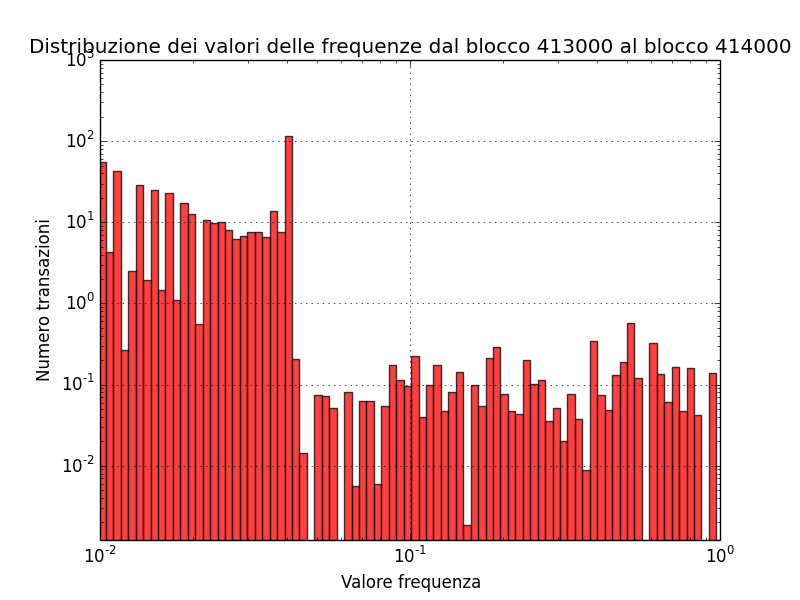
\includegraphics[width=\textwidth]{figure/hist1000b}
	\caption{\textit{1000 blocchi}\label{fig:hist1000b}}
\end{figure}

\begin{figure}
	\centering
	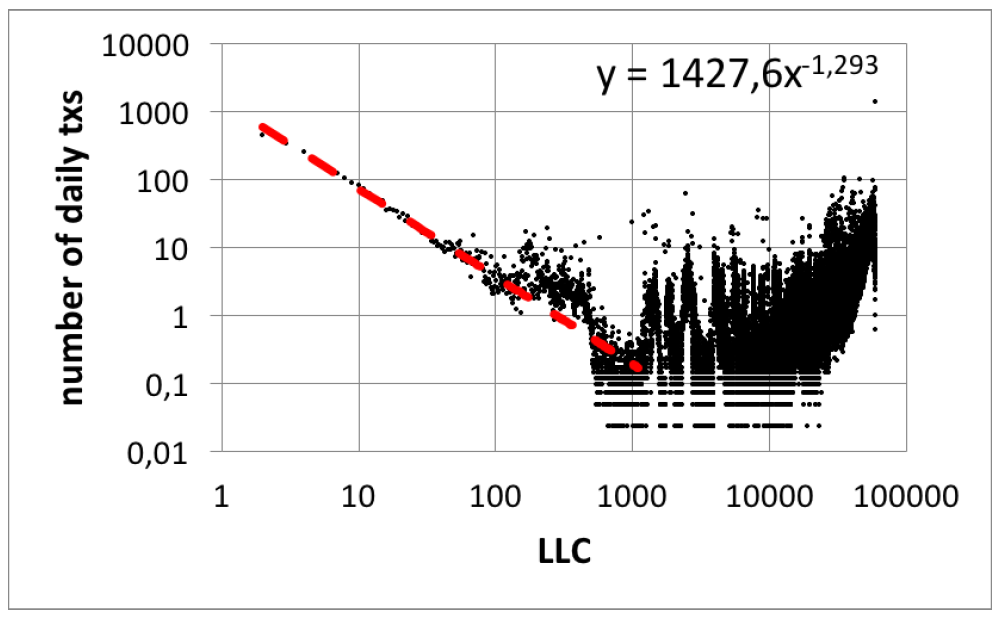
\includegraphics[width=0.6 \textwidth]{figure/graphpaper}
	\caption{\textit{Grafico di valori llc \cite{ddp-ltcbh-17} }\label{graphpaper}}
\end{figure}

\subsection{Al variare del parametro p}

Un'altro metodo di studio delle catene di transazioni, è stato quello di calcolare la frequenza facendo intervenire un parametro $p$.

Esso corrisponde al numero degli ultimi elementi della catena di transazioni su cui viene calcolata la frequenza media. Infatti, secondo l'algoritmo, inizialmente vengono assegnati dei valori arbitrari ai nodi iniziali delle chain. Successivamente, tramite la visita delle varie catene, il valore si modifica gradualmente. Quello che interessa maggiormente è il valore di frequenza calcolato sugli ultimi $p$ elementi, in modo da estrapolare solamente ciò che più caratterizza tale catena.

Gli esperimenti e i grafici fatti finora avevano come parametro p=100. Nella figura \ref{fig:p50} si può notare la distribuzione del grafico con p=50.

\begin{figure}[htbp]
	\centering
	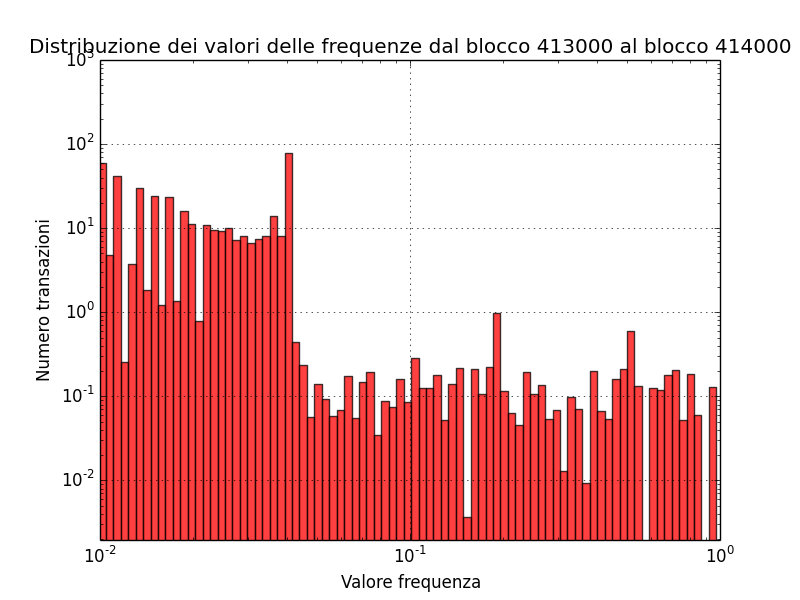
\includegraphics[width=0.8 \textwidth]{figure/p50}
	\caption{\textit{1000 blocchi con p = 50}\label{fig:p50}}
\end{figure}

\section{Discussione dei risultati}
Nel paragrafo precedente sono stati messi a confronto i risultati ottenuti nell'esecuzione dell'algoritmo, con il grafico del paper \cite{ddp-ltcbh-17}. 

I grafici generati dall'algoritmo in questione vengono rappresentati tramite istogrammi. La scala che si è preferita utilizzare è una scala logaritmica, sia sull'asse x che sull'asse y, poiché riesce ad evidenziare meglio le peculiarità e gli andamenti rilevanti che altrimenti non sarebbero identificabili su una scala standard.

I singoli bucket che costituiscono gli istogrammi sono stati disegnati secondo una loro scala logarimica in modo da farli apparire tra di loro equivalenti. 

I due grafici messi a confronto, condividono un andamento comune, ossia un andamento iniziale verso il basso. Tale pendenza si riscontra quindi, non solo sui valori della frequenza assegnata dall'algoritmo, ma anche sui valori di LLC del secondo grafico. In questo modo si potrebbe esprimere un collegamento tra i valori di frequenza e i valori di llc, che verrà lasciato come spunto per gli sviluppi futuri.

Dal momento che il valore di llc assegnato ad un nodo esprime la lunghezza del cammino più lungo di cui esso fa parte, si potrebbe sostenere che all'aumentare del valore di llc, i nodi che hanno quel valore, diminuiscono. Ossia, più aumenta il parametro, meno sono i nodi a cui corrisponde tale quantità.

Questa caratteristica si può notare anche nel grafico delle frequenze in cui, più aumenta la frequenza, meno sono i nodi con quel valore.

Nella parte destra, i due grafici differiscono. Infatti nel primo, i valori sembrerebbero seguire un andamento medio costante. Nel secondo invece, l'andamento sembra crescere gradualmente. 

E' probabile che quindi ci siano delle discrepanze per quanto riguarda i dati, o l'approccio dettato dagli algoritmi. Ma, prendendo in considerazione quanto visto in precedenza, si potrebbe pensare che non esiste, in questo caso, nessun tipo di corrispondenza tra i due parametri(frequenza ed llc).

Nel primo grafico \ref{fig:hist1000b} è probabile che la frequenza segui un andamento pressoché costante, infatti all'aumentare del valore, si hanno quasi sempre lo stesso numero di nodi che hanno quella frequenza.

Nel secondo grafico \ref{graphpaper} all'aumentare di llc, esistono più nodi che hanno quel valore. Dal momento che il parametro llc rappresenta il numero di nodi che fanno parte della catena più lunga di appartenenza del nodo corrente, si potrebbe pensare che questo è dato dal fatto che, essendoci tanti nodi facenti parte di una singola catena lunga, essi andranno a rimpolpare le fila dei nodi con quel valore di llc per quella catena lunga. In poche parole, se si ha una chain di transazioni di 100 nodi, si avranno almeno 100 nodi con il valore di llc pari a 100. Di conseguenza il motivo per cui si ha quel picco crescente, è evidentemente influenzato dal parametro stesso.

Infine, non si nota una particolare equivalenza di valori, prendendo in considerazione anche gli intervalli degli assi, che chiaramente non sono equivalenti.

Per quanto riguarda il dataset, invece, nei grafici prodotti dall'esecuzione di questo algortimo, non si nota un cambiamento al variare del dataset. Infatti, se si varia la dimensione del dataset, si può notare che il grafico va ad infittirsi, ma l'andamento rimane sempre lo stesso. 

Nel paper preso in considerazione, è stato utilizzato lo stesso approccio: variare la dimensione del dataset al fine di mantenere invariato il grafico finale. Purtroppo ciò non è accaduto, infatti dalla figura \ref{papergraph2}, si evince che all'aumentare dei dati, la curva maggiore trasla di un certo numero di valori.

Ogni curva ha un colore poiché ogni curva rappresenta un certo intervallo di blocchi preso come input. Sull'asse x c’è il valore di LLC e sulle y c’è il numero di istanze che hanno quell’LLC.
\newpage
Il codice dei colori dell'immagine, rappresenta i seguenti intervalli di dataset:
\begin{itemize}
\item 413000_413191 -> nero
\item 413000_413383 -> rosso
\item 413000_413767 -> giallo
\item 413000_414535 -> blu
\item 413000_416071 -> viola
\item 413000_419143 -> arancione
\end{itemize}


\begin{figure}
	\centering
	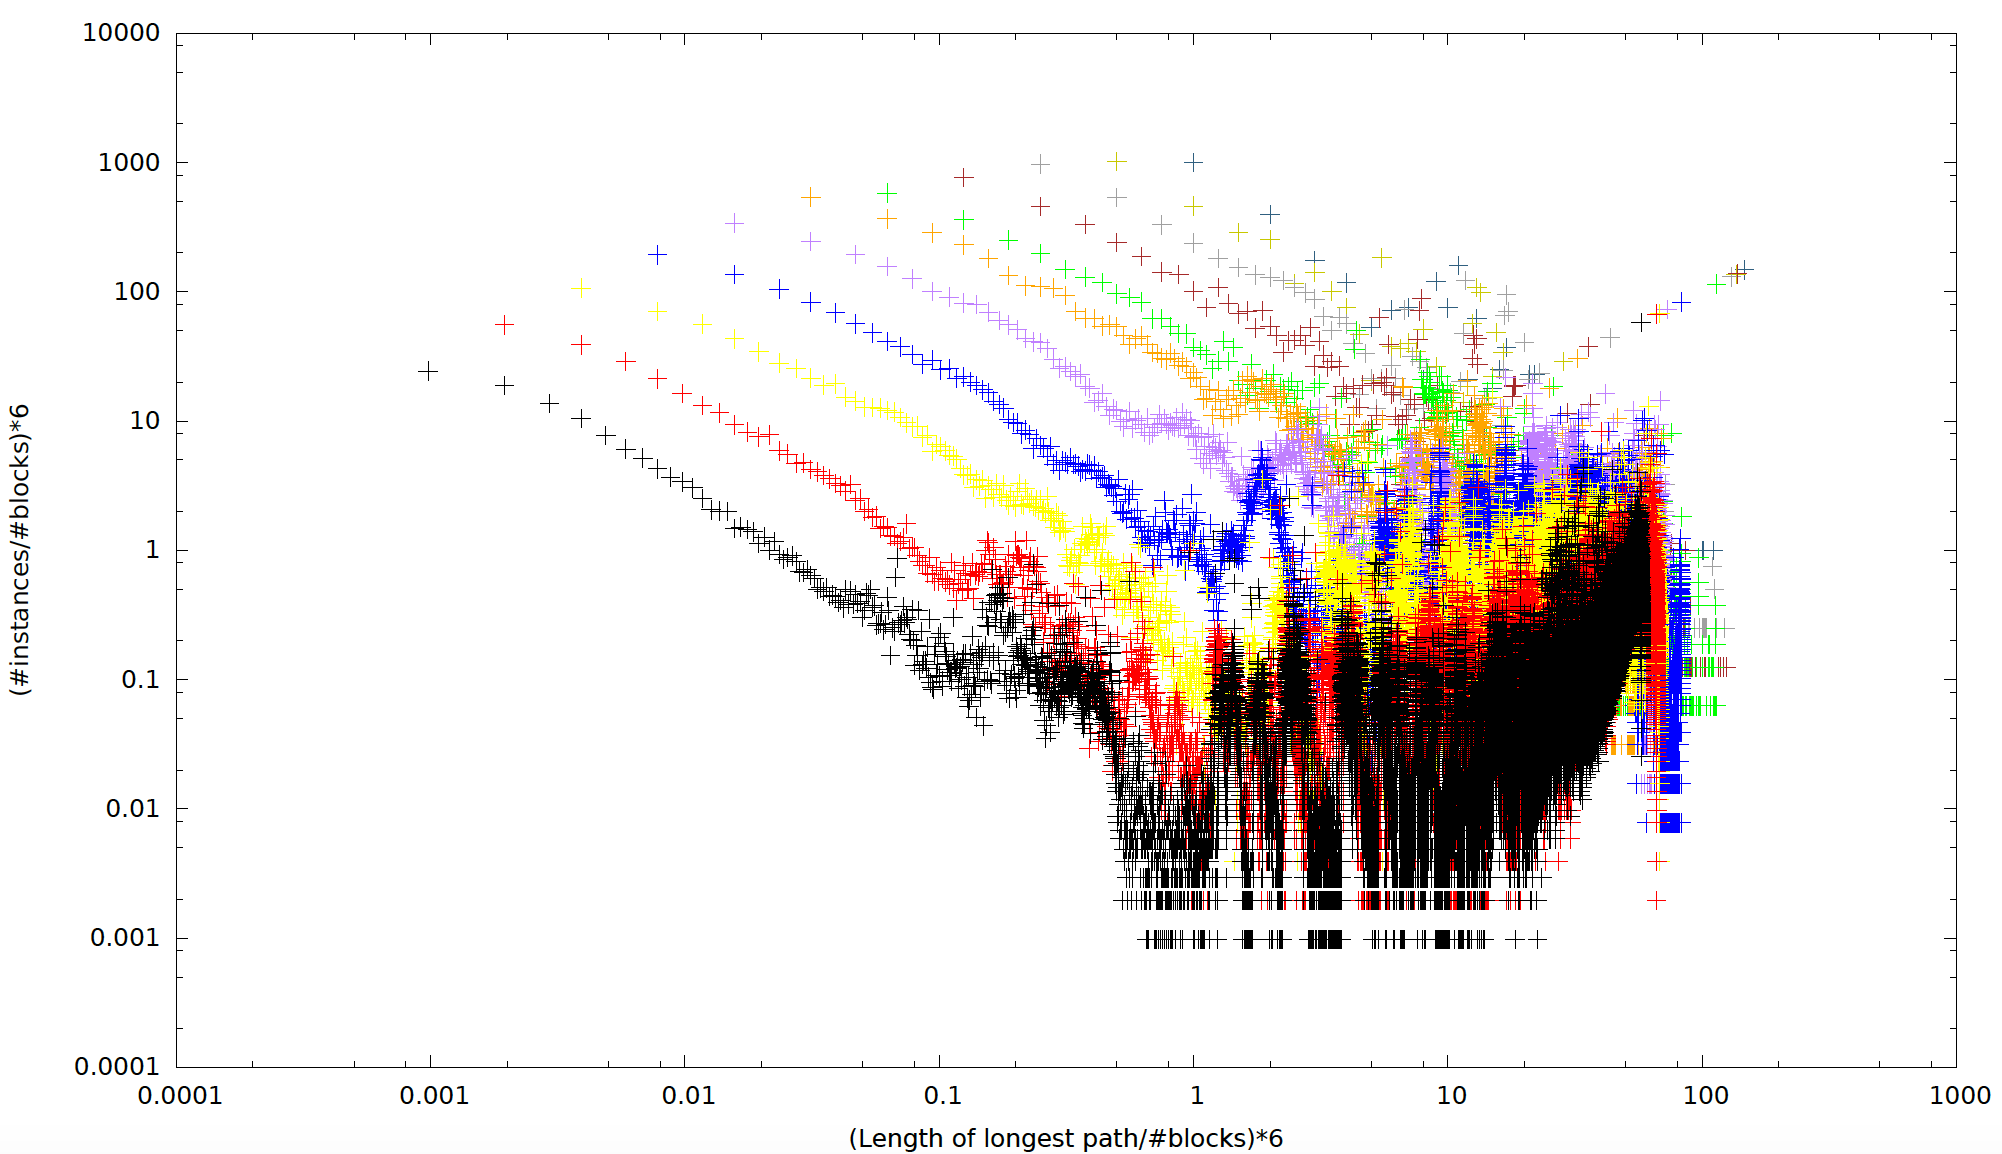
\includegraphics[width=\textwidth]{figure/papergraphlogscale}
	\caption{\textit{Grafico di valori llc al variare del dataset \cite{ddp-ltcbh-17} }\label{papergraph2}}
\end{figure}

Si osserva che la curva cambia in relazione al cambiamento della dimensione dell'input, diversamente da quanto viene mostrato nei grafici delle pagine precedenti.

Per quanto riguarda invece, il parametro p, esso non interviene nella trasformazione del grafico; infatti, sia con p=100 che con p=50 il risultato è quasi lo stesso. 
Quindi, il parametro p non influenza direttamente i dati e i risultati dell'esperimento.